\documentclass[11pt, a4paper]{article}
\usepackage[margin=2.5cm]{geometry}
\usepackage{polyglossia}
\setdefaultlanguage[spelling=new]{german}
\usepackage{amsmath}
\usepackage{graphicx}
     
\begin{document}

%%// INSERT typing
%% https://en.wikipedia.org/wiki/Jessie_Craigen
It is not certain where in the UK she was born, although the Dover Express
in 1866 described her as a 'Scotch lady'. The 1871 census, however, shows
her living with an adopted 18-year-old child, Rosetta Vincent, and a married
sister, Emma Henley, in Ordsall near Retford and describing herself as a ‘lecturer’,
born in London. By 1881 she is in Clifton, Bristol, and in the census she
describes herself as a London-born, ‘Lecturer on Social Subjects’.

She reportedly had a seafaring father from the Scottish Highlands,
who died when she was an infant, and a mother who was an Italian actress.
As a child she appeared on the stage and this may have given her the skills
and the confidence for paid public speaking.
%%// END
%% at the start

\textbf{Technische Universität Berlin}\hfill\textbf{WiSe 2019/2020} \\
\textbf{Fakultät II, Institut für Mathematik}\hfill\textbf{Woche 3} \\
Sekreteriat MA \\
Dr. Max Mustermann \\
Ola Nordmann, John Doe

\vspace{.5cm}
\raggedright

\begin{center}
    {
        \Large
        \textbf{3. Übungsblatt Computerorientierte Mathematik II}
    }
    \large
    
    \vspace{.25cm}
    
    \textbf{Abgabe: 03.05.2019} (bis 10:10 Uhr in MA 001)
    
    \vspace{.25cm}
    
    \textbf{Alle Antworten sind zu beweisen.}
\end{center}

\section*{1. Aufgabe\hfill\textnormal{\normalsize (1 + 1 + 2 Punkte)}}
Ein \emph{Binärbaum} ist ein Wurzelbaum, in dem jeder Knoten $\leq 2$ Kinder hat.
Die Tiefe eines Knotens $v$ ist die Länge des eindeutigen Weges von der Wurzel
zu $v$, und die Höhe von $v$ ist die Länge eines längsten (absteigenden) Weges
von $v$ zu einem Blatt. Die Höhe des Baumes ist die Höhe der Wurzel.

\vspace{6mm}

\begin{center}
    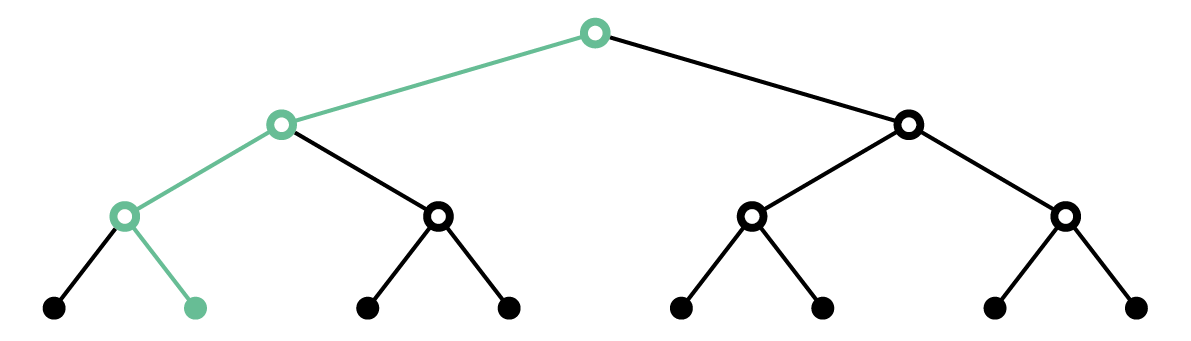
\includegraphics[width=.9\textwidth]{../assets/graph}
\end{center}

Berechnen Sie, wie viele Kanten maximal begangen werden müssen, um in einem Wurzelbaum mit der Tiefe $v$ von einem gegebenen Knoten jeden anderen Knoten zu erreichen. Beweisen Sie Ihr Ergebnis nach dem in der Vorlesung besprochenen Schema.

\section*{2. Aufgabe\hfill\textnormal{\normalsize (2 + 1 + 5 Punkte)}}

Ein \emph{primes} Element eines Zahlenkörpers teilt das Produkt $ab$ genau dann, wenn es entweder $a$ oder $b$ teilt.

\begin{enumerate}
    \item Beschreiben Sie, wie sich ein primes Element und eine Primzahl unterscheiden? (2 Punkte)
    \item Hat jeder Zahlenkörper, der Primzahlen enthält, auch prime Elemente? (1 Punkt)
    \item Beweisen Sie, dass die Polynome $x^2 - 2$ und $x^2 + 1$ in $\textbf{Z}[x]$, dem Ring der Polynome über $\textbf{Z}$, Primelemente sind.
\end{enumerate}
\end{document}
